\begin{figure*}[htbp!]
	\centering
	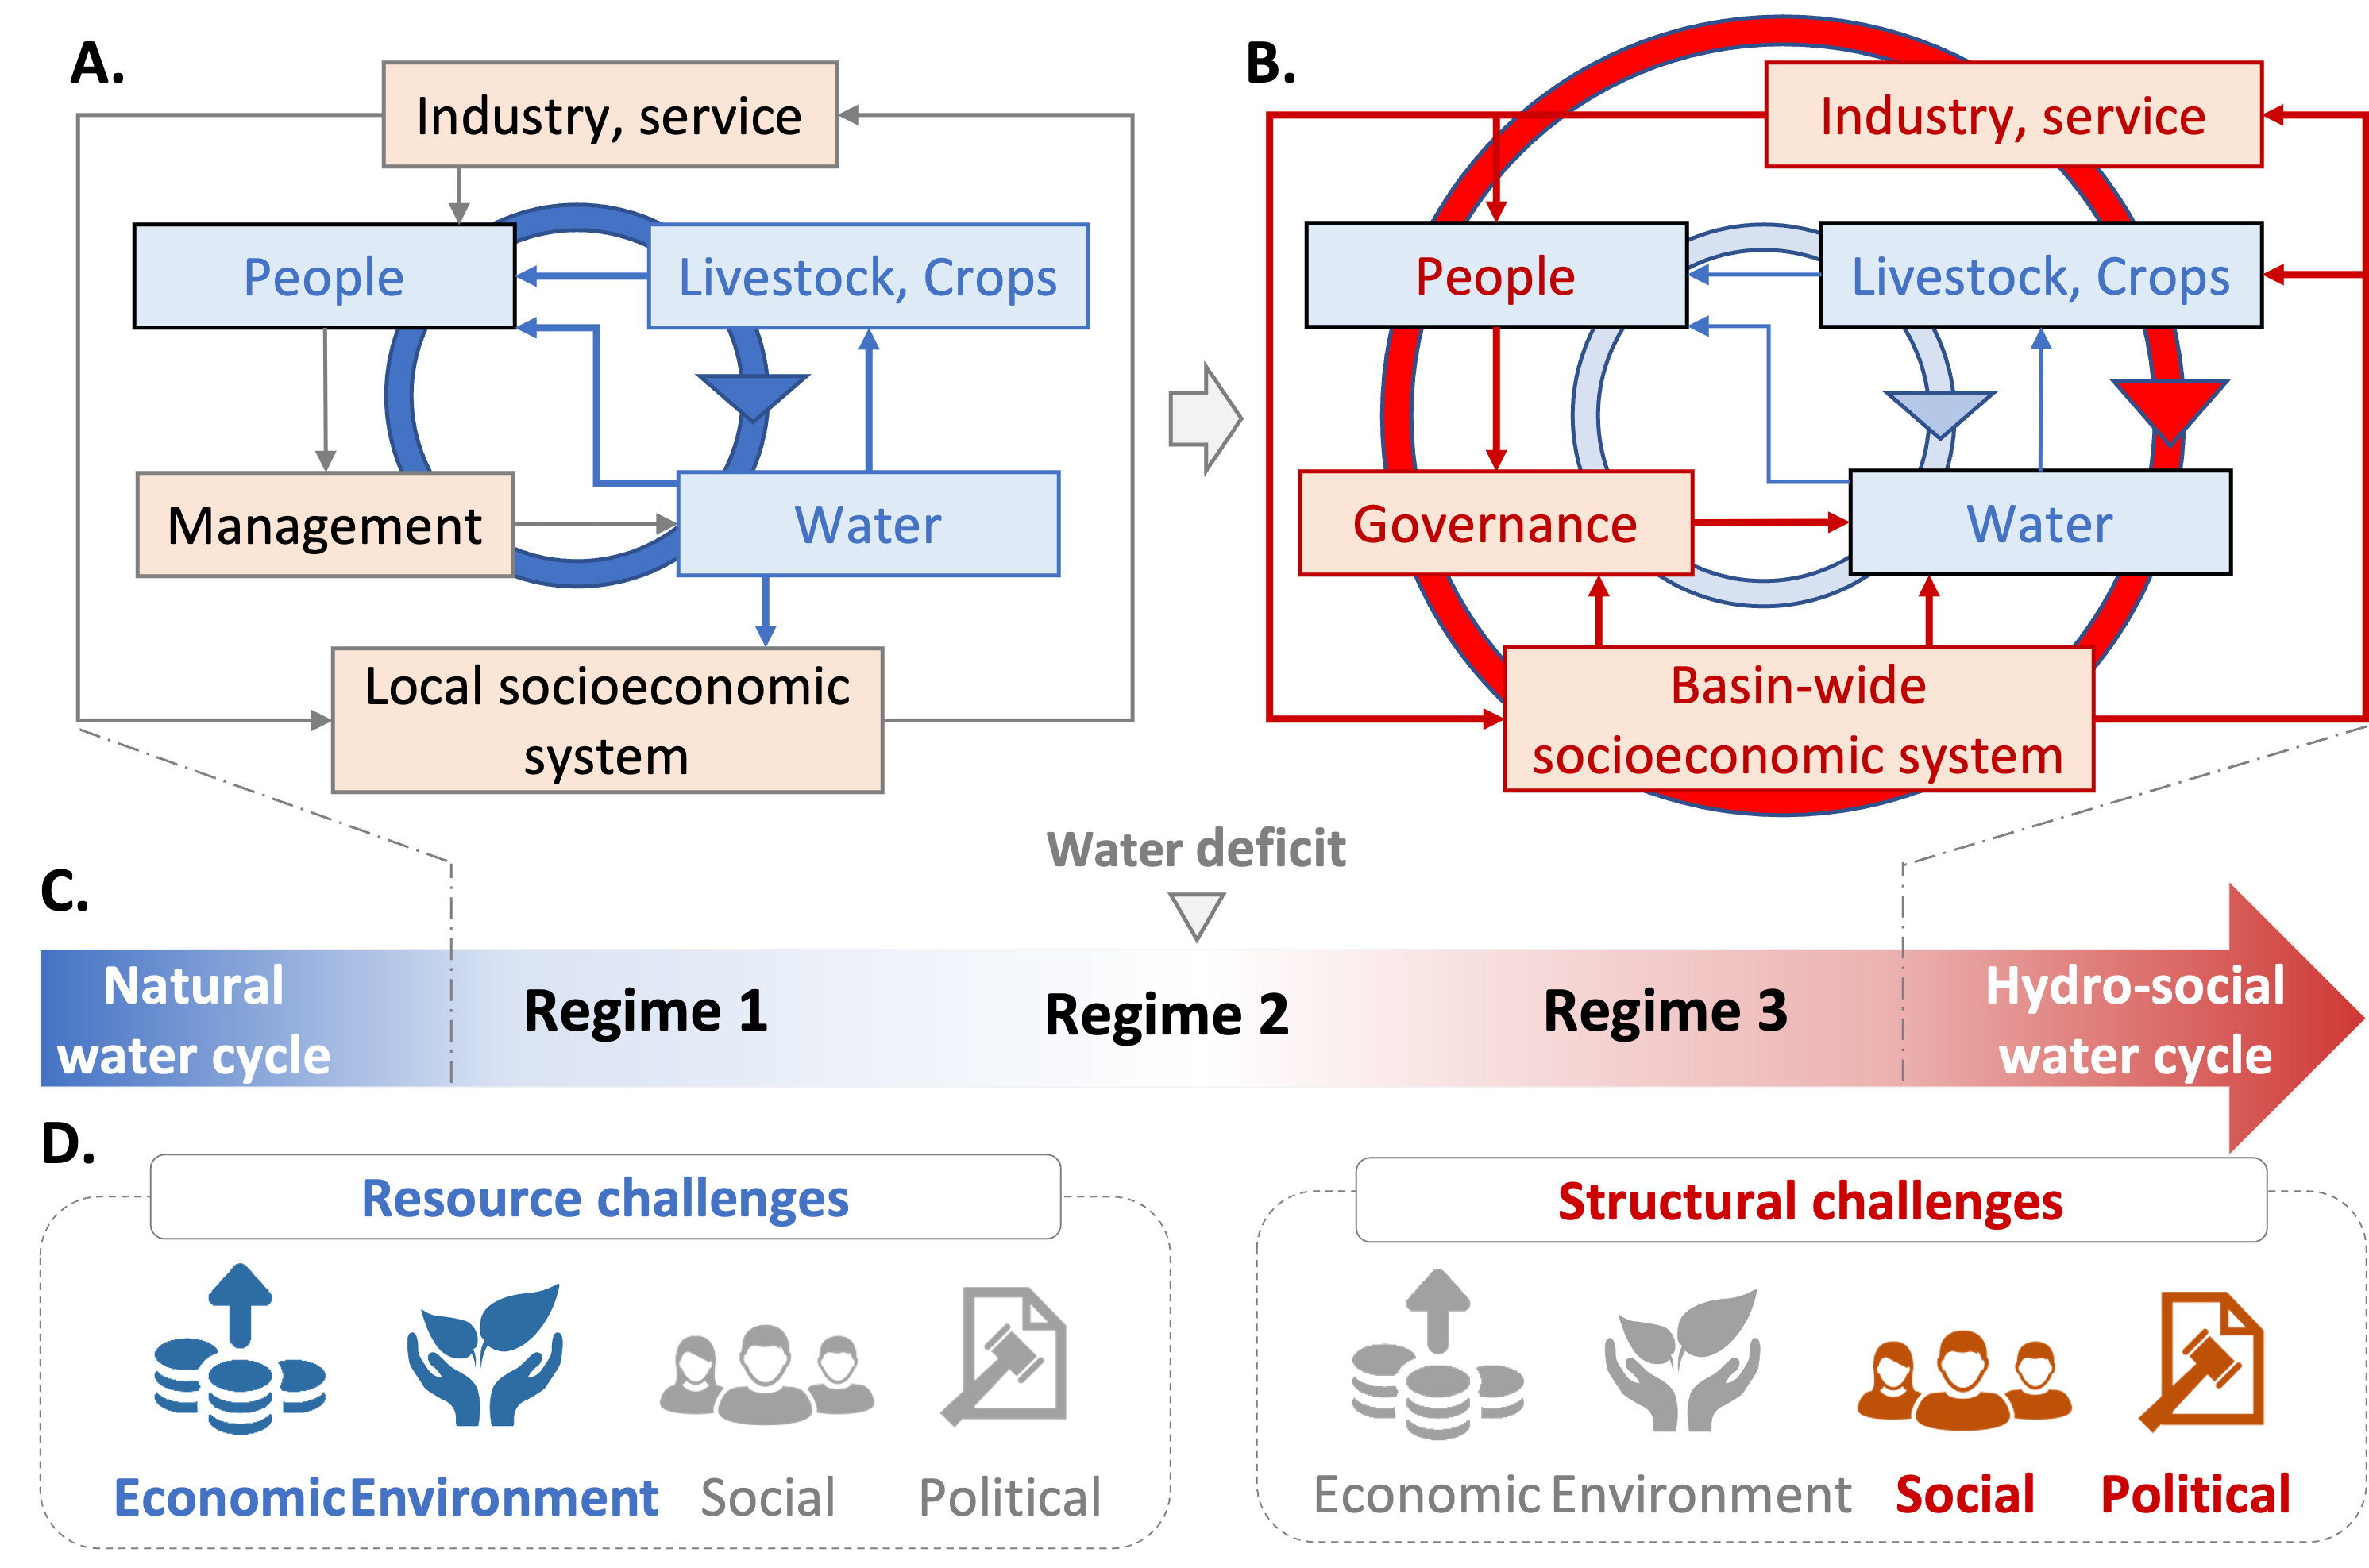
\includegraphics[width=0.9\linewidth]{main/transition.png}
	\caption{
		Transition schema in hydrosocial cycle and water governance regimes. The natural water cycle dominates blue pathways, while socio-economic feedback dominates red pathways.
		\textbf{A.} As socio-economic systems develop, non-provisioning water demand increases; simultaneously, increased adaptive capacity by engineering allows people to manage water resources to alleviate the water stress.
		\textbf{B.} With further human interventions, trade-offs between provisioning-purpose and non-provisioning water use become prominent; a basin-wide socio-economic system requires more organized water governance.
		Thus, \textbf{C. the hydrosocial water cycle transition} correlates with the water governance regime shifts (in the YRB, they are massive supply regime, transformation governance regime, and adaptation oriented regime). The transformation governance regime shift occurs following the water deficit, with the rapid growth of adaptive capacity.
		\textbf{D. Water governance challenges} Through the transitional regimes, water governance faces primarily economic and environmental challenges but social and policy challenges later.
	}
	\label{fig:summary}
\end{figure*}

% Implications
Water governance gradually becomes a national or international concern from a primarily local concern because large river basins are critical sources of ecosystem services, economic development, and human well-being
\cite{best2019,best2020}.
As the ubiquitous tele-coupling is rising additional water governance challenges in the tighter connected world, the transition of hydrosocial cycle and regime shifts align with different human-water relationships \cite{diaz2019}.
The process echoes how societies can change governance practices by enhancing their adaptive capacity in the hydrosocial cycle, and the IWGI quantitatively identifies this transition \cite{loch2020,turton1999}.
It is vital for scientists and decision-makers to recognize the changing governance challenges because models, institutions, engineering, and approaches developed under one regime are not necessarily applicable under a different regime \cite{reyers2018}.

% 我们为的研究结果表明,黄河流域能被识别为三个明显的稳态。
In the case of the YRB, our results show that there have been three distinct but sequential governance regimes: a massive supply regime (P1: 1965-1978), a governance transforming regime (P2: 1979-2001) and an adaptation oriented regime (P3: 2002-2013).
During the massive supply regime with lower water stress (1965-1978 in the YRB), water governance thus tended to boost water supply for services (mainly provisioning purposes then -livestock and crops) by constructing reservoirs and channels.
As the popular slogan ``man will conquer nature'' suggested, however, the enhancement of water supply aligned with little consideration of the irreversible changes in the human-water relationship, thus drastically increasing water demand with little consideration in basinal conservation
\cite{zhou2020}.
The rapid expansion of irrigated farmland and water diversion facilities in that decade brought the overburdened YRB close to the critical point, where keeping increasing supply to meet the unlimited demand is unpractical \cite{loch2020}.
As a result, the over 80\% surface water use then led to river depletions frequently since 1972, with ecological issues, such as wetlands shrinkage and declines in biodiversity \cite{wang2019c}.
In addition, as the water stress also limited the industrial economy in the ascendant, the existing modes of water governance led to a social-ecological crisis and challenged sustainability rigorously
\cite{wohlfart2016a}.

The start of the governance transforming regime (P2: 1979-2001) coincided with the rising competition for water use after the ``reform and opening-up''.
% 正如理论预测的那样
The results in the YRB keep in line with the suggestions from the theoretical analysis: continuous increases in water demand when the basinal total supply is stable can follow substantial changes in governance regime and the rapid enhancement in overall social adaptive capacity \cite{loch2020}.
% 作为制度转变的先行者
Being a pioneer in shifting governing institutions, the YRB triggered a series of changes in ``who gets water, when and how'' during this regime: slowing growth of irrigated acreage; leading water-saving infrastructure; China's first water quota scheme; The preliminary cross-boundaries water transfer plan and so on
\cite{wang2019a,long2020,nickum2021}.
% 因此,1999年黄河的最后一次枯竭
Consequently, though water stress remained and increased (mainly led by reducing streamflow and flexibility), the last depletion of the Yellow River in 1999 added a footnote to the climax of this transformation in water governance \cite{wang2019a}.

When it came to an adaptation-oriented regime (P3: 2002-2013), drastically shifting in societies adapted to the stable high water stress.
Socio-economic trade-offs between water-dependent regions and sectors played a more important role in this regime, so water governance had to achieve efficient water allocation while balancing different purposes in the face of limited water supply
\cite{dalin2015,song2022}.
Reconstruction of resources widespread in different industries and regions was calling for adaptation in water governance, where the urgent requirements of adjusting the rigid quota shares from the previous regime can be an example \cite{wang2019a}.
Like this, many national-level governing practices were proposed under the regime because the absence of such policies with the social dilemma of high-quality development became new structural challenges for water governance
\cite{konar2019}.

% 总体而言,长江流域的水治理是“改善供给、转变治理、增强适应”的水社会循环总体转型中最突出的例子之一。
In general, water governance of the YRB is among the most prominent example in the general transition of hydrosocial cycle -``improving supply, transforming governance, and enhancing adaptation''.
With each dimension changing gradually, the emergence of regime shifts drives the water governance challenges at a basin-scale: primarily economic and environmental before the transformation but social and policy-related towards the end (Figure~\ref{fig:summary}) \cite{singh2019,porcher2019}.
In the analogy at a global scale, the resource challenges, represented as water shortage and water supplying difficulties, are mainly faced by undeveloped and developing basins
\cite{allan2019,speed2013,liu2012a}.
Alternatively, highly-controlled and developed basins (especially for transboundary rivers) must mainly resolve structural challenges, such as water disputes or lack of equity, and may be in urgent need of novel flexible, efficient sociopolitical governance structures %* Kitroeff citation wrong
\cite{unep-dhi2016,mirumachi2015}.
Linking regime shifts to the governance challenges, the implementation of IWGI thus offers a comprehensive and straightforward way to interpret the intertwines between water governance and the hydrosocial transition.

%* limitations & direction
One of the main limitations in the approach is the few data worldwide with a long-term period, which means still a gap between the comprehensively identifying and widespread application of IWGI.
However, we assumed that all water governance issues are relative to ``who gets water, when and how'', so water stress, purposes of water services, and water allocation patterns matter.
Therefore, we suggest that choices of the indicators for the dimensions can be adapted according to available datasets as the intertwines between the underlying components are much more crucial in understanding the transition of governance regimes holistically.
In today's world, the regime shifts from biophysical to hydrosocial control of dynamics may become increasingly widespread, so the comprehensive strategies to address governance challenges have become the core of complex human-water systems
\cite{cumming2018,cumming2014,jaeger2019}.
Although river basins have shown improvements in water management technologies and water use efficiency, many of them are still approaching planetary boundaries where human-water systems may collapse
\cite{gleeson2020, wang-erlandsson2022}.
A deeper understanding of governance that incorporates ideas of non-linear regime shifts and transformations should help shift the focus of governance towards maintaining the resilience of the basin’s social-ecological system and improving its sustainability
\cite{falkenmark2019}.
